\section{Absicherung}

\subsection{Architektur und Design}

\subsection{LISP Map Server}
Es gibt zwei Betriebsarten für einen LISP Map-Server(MS): 
\begin{itemize}
	\item als Map-Resolver(MR), der Map-Requests von einem ITR entgegennimmt und das EID-zu-RLOC-Mapping mit Hilfe der verteilten Mapping-Datenbank auflöst
	\item als Map-Server(MS), der autoritative EID-zu-RLOC-Mappings von einem ETR lernt und in der Datenbank veröffentlicht
\end{itemize}


\subsubsection{Redundante MS / MR Bereitstellung}

Es wird empfohlen, redundante eigenständige MS- und MR-Systeme mit den MS / MR-Funktionen auf demselben Gerät bereitzustellen. Wenn redundante eigenständige MS / MR implementiert werden, müssen sich alle xTRs bei beiden MS registrieren, so dass jeder eine konsistente Sicht auf den registrierten LISP EID-Namespace hat. Für Map-Resolver-Funktionalität ist die Verwendung einer Anycast-IP-Adresse wünschenswert, da dadurch die Mapping-Lookup-Leistung verbessert wird, indem der MR ausgewählt wird, der dem anfordernden ITR am nächsten ist.

\begin{figure}[H]
	\centering
	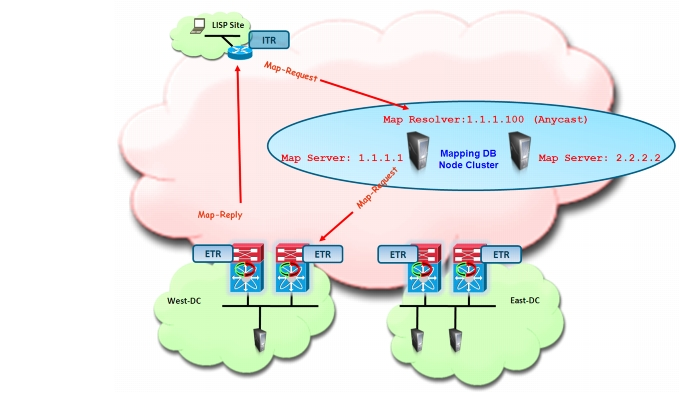
\includegraphics[width=1\linewidth]{img/Analyse/LISP-Example}
	\caption{Redundante MS / MR Bereitstellung \cite{LISP-mobility} }
	\label{fig:Redundante MS / MR Bereitstellung}
\end{figure}

\subsubsection{Co-Lokalisierung von MS / MR und xTR Funktionalitäten}

Ein weiteres Beispiel ist die Co-Lokalisierung  von MS / MR- und xTR-Funktionalitäten. Das oben gezeigte co-lokalisierte Modell ist besonders vorteilhaft, da es die Gesamtzahl verwalteter Geräte reduziert, die zum Ausrollen einer LISP Host Mobility-Lösung erforderlich sind. Es muss beachtet werden, dass die erforderliche Konfiguration in beiden Szenarien identisch bleiben würde, indem eindeutige IP-Adressen verwendet werden, um die Map-Server und eine Anycast-IP-Adresse für den Map-Resolver zu identifizieren.

\begin{figure}[H]
	\centering
	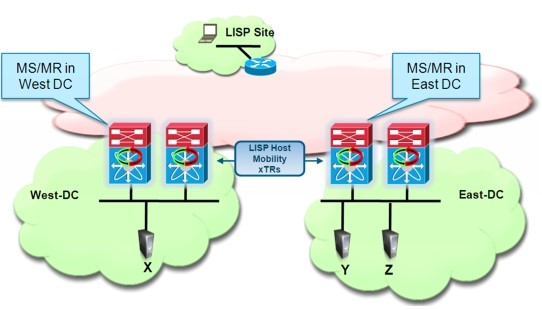
\includegraphics[width=0.8\linewidth]{img/Analyse/LISP-Example2}
	\caption{Co-Lokalisierung von MS / MR und xTR Funktionalitaeten \cite{LISP-mobility} }
	\label{fig:Co-Lokalisierung von MS / MR und xTR Funktionalitaeten}
\end{figure}

Es kann also ein redundantes eigenständiges MS / MR-Modell bereitgestellt werden, indem dedizierte Systeme zur Durchführung dieser Mapping-Funktionen genutzt werden (siehe Abbildung 2.9) oder alternativ können die MS- und MR-Funktionen gleichzeitig auf dem Netzwerkgerät, welches bereits die xTR-Rolle ausführt, implementiert werden (siehe Abbildung 2.10).

\subsection{ISE / Radius}

\subsubsection{ISE Cluster}

Um die Verfügbarkeit des ISE zu erhöhen, kann diese in einem Cluster, bestehend aus einem Master und mehreren Slaves betrieben werden. Dies erhöht die Ausfallsicherheit aller Services auf dem ISE. Damit diese gewährleistet sind, wenn ein Aussenstandort die Verbindung zum Hauptsitz verliert, müsste aber an jedem Standort ein ISE Slave existieren. Bei sehr vielen Standorten ist dies auf Grund des Verwaltungsaufwands und der Kosten für viele ISE Instanzen nicht praktikabel. Ein Cluster am Hauptstandort ist aber sicherlich sinnvoll.

\subsubsection{Read Only Radius Server an Aussenstandorten}

In Aussenstellen wird ein Read Only Radius Server betrieben, damit die Network Access Devices auch im Falle eines Unterbruchs der Verbindung zum Hauptsitz einen Radius Server zur Verfügung haben. Hier könnte beispielsweise Freeradius eingesetzt werden. Da Freeradius seine Informationen nicht direkt vom ISE beziehen kann, muss vom ISE ein externer Radius Server verwendet werden, der eine Replikation unterstützt. Dies kann beispielsweise Freeradius sein.

\paragraph{ISE}


\paragraph{Freeradius}

Freeradius wird in einem Master / Slave Setup betrieben. Am Hauptstandort befindet sich der Radius Master und an allen Aussenstandorten ist ein Slave verfügbar. Die Replikation wird mittels MySQL Replikation sichergestellt.

\paragraph{Network Access Devices}

Auf den Network Devices muss der Radius Server vom jeweiligen Standort konfiguriert sein. Dies kann im DNA Center unter \textit{Design $\rightarrow$ Network Settings $\rightarrow$ AAA Server} konfiguriert werden.

\begin{figure}[H]
	\centering
	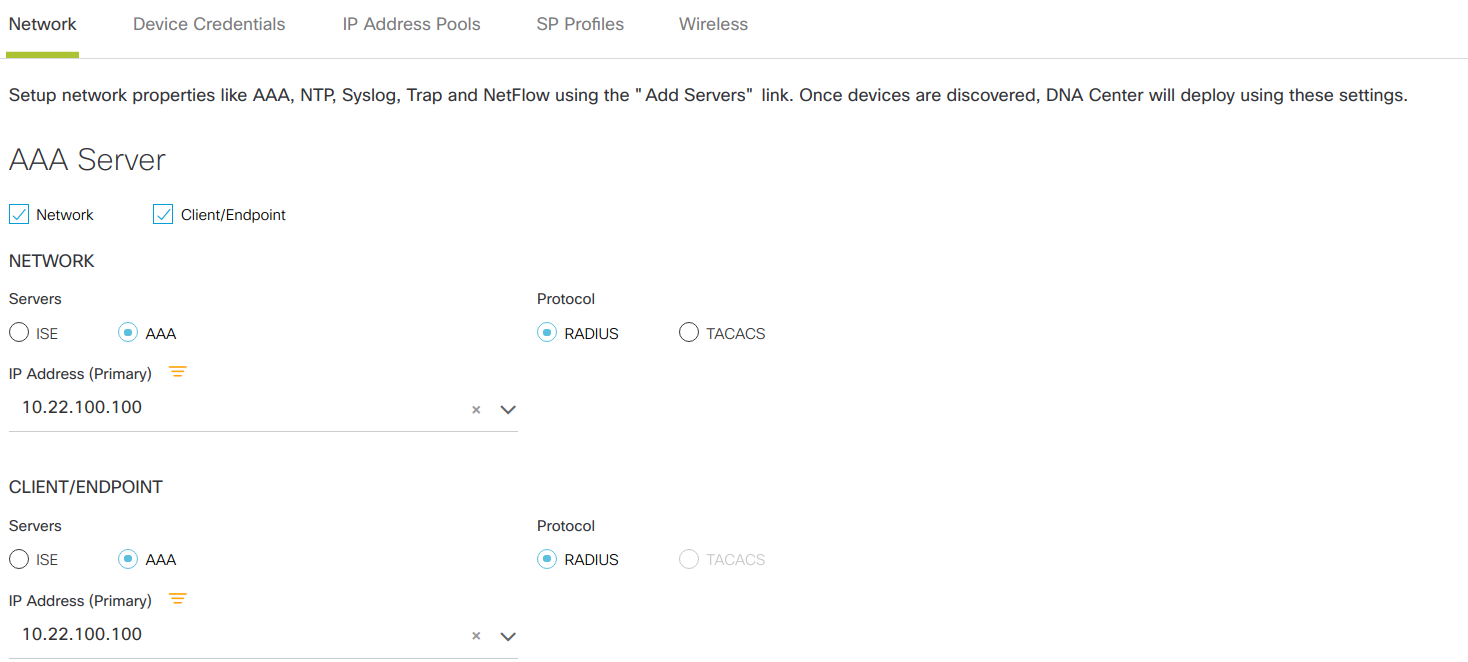
\includegraphics[width=0.8\linewidth]{img/Absicherung/DNA_Center_AAA-Server.png}
	\caption{DNA Center - AAA Server }
	\label{fig:DNA Center - AAA Server}
\end{figure}


\subsection{SGT Access List}

\subsection{Border Node}

\subsection{Fusion Router}

Es werden mehrere Fusion Router verwendet, um die nötige Ausfallsicherheit zu gewährleisten. Die Fusion Router und Border Nodes sind im Optimalfall in einem Full-Mesh verkabelt. Für das Routing zwischen den Fusion Routern, sowie den Border Nodes kommt BGP zum Einsatz.

\subsection{DHCP}

\subsection{DNS}

\subsubsection{Infoblox HA Cluster}


\subsubsection{Read Only DNS Server an Aussenstandorten}
	
Damit Aussenstellen nicht auf DNS Server des Hauptstandortes angewiesen sind, kann in jedem Standort ein Read-Only Server betrieben werden. Somit funktioniert die Namensauflösung auch im Falle eines Kommunikationsverlusts zum Hauptstandort. 

\begin{figure}[H]
	\centering
	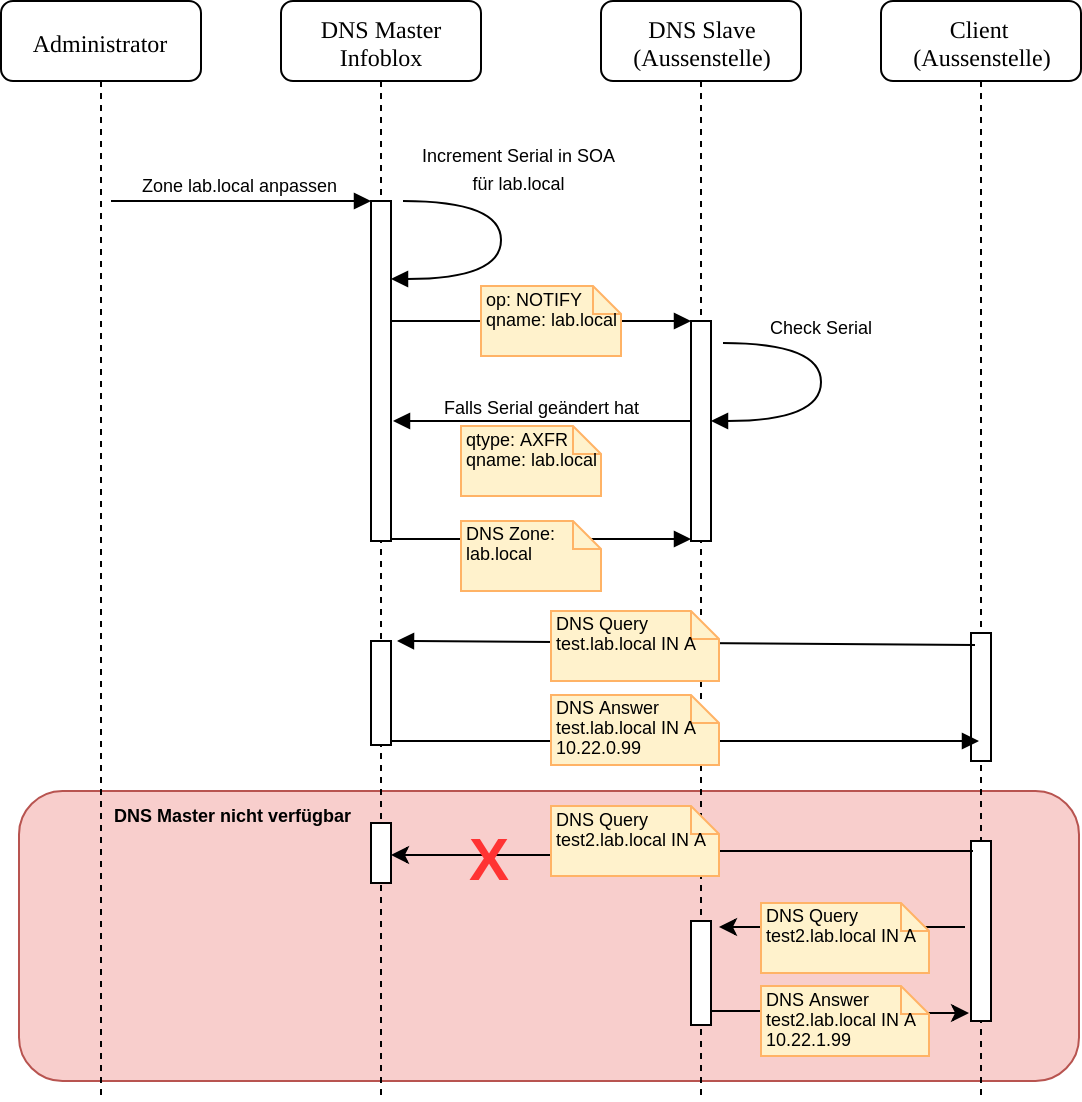
\includegraphics[width=0.8\linewidth]{img/Absicherung/DNS_Sequenzdiagram.png}
	\caption{DNS Sequenzdiagramm}
	\label{fig:DNS Sequenzdiagramm}
\end{figure}
\paragraph{Infoblox}

Damit die Read-Only Server stets über die aktuellsten DNS Zonen verfügen, müssen die Informationen von Infoblox auf diese repliziert werden. In diesem Fall wird dafür der Zone Transfer verwendet. Dazu muss dies in Infoblox für alle Slave Server erlaubt werden. 

Dies wird in Infoblox via \textit{Grid $\rightarrow$ DNS $\rightarrow$ Infoblox Instanz $\rightarrow$ Edit $\rightarrow$ Zone Transfers} ausgeführt.

\begin{figure}[H]
	\centering
	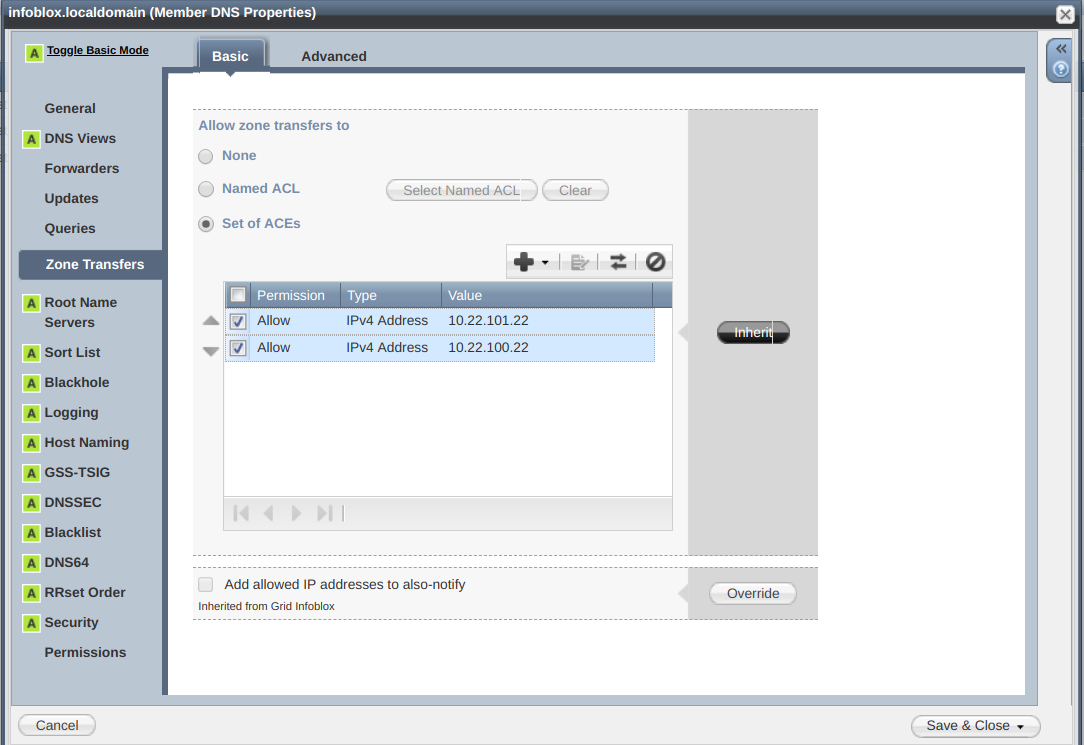
\includegraphics[width=0.8\linewidth]{img/Absicherung/Infoblox_Zone_Transfer.png}
	\caption{Infoblox Zone Transfer}
	\label{fig:Infoblox Zone Transfer}
\end{figure}

\paragraph{DNS Slaves}

Auf den Slaves an den jeweiligen Aussenstandorten müssen die Zonen als Slave Zonen konfiguriert sein und Infoblox muss als Master konfiguriert werden. Dadurch können die Zonen vom Master auf den Slave transferiert werden. Der Slave aktualisiert alle Slave Zonen in regelmässigen Abständen. Dieser Intervall wird in der Zone im SOA Record mit dem "Refresh" Parameter definiert.
Zusätzlich kann auf dem Master konfiguriert werden, dass alle Slaves mittels "Notify" informiert werden, sobald sich eine Zone ändert, worauf der Slave die aktuellsten Informationen für diese Zone abruft. Somit ist sichergestellt, dass alle Server an Aussenstandorten stets über eine aktuelle Konfiguration verfügen.

\paragraph{Clients}

Auf den Cliens ist es wichtig, dass alle nötigen DNS Server in der korrekten Reihenfolge konfiguriert werden. Als erster Server soll der Master, also Infoblox eingetragen werden. Sofern Infoblox als Cluster betrieben wird, können auch alle Instanzen des Clusters verwendet werden. Danach der Slave am jeweiligen Standort. Dies sorgt dafür, dass der Slave nur dann verwendet wird, wenn die Kommunikation zum Master nicht funktioniert.